% =====================================================================
%  Ingenieria de Requisitos (ISR-401) -- UTEQ
%  Facultad de Ciencias de la Ingenieria -- Carrera de Ingenieria de Software
%  PRUEBA PRACTICA -- UNIDAD IV: Validacion, Gestion, Herramientas y Estandares
%  PARALELO B -- Caso: Sistema de Reserva de Citas Medicas.
%  Modalidad: individual, en clase, con repositorio.
%  Documento autonomo compilable. Formato tipo libro, A4.
%  Compilacion:  pdflatex main -> bibtex main -> pdflatex main -> pdflatex main
% =====================================================================
\documentclass[11pt,a4paper,oneside]{article}

\usepackage[utf8]{inputenc}
\usepackage[T1]{fontenc}
% Nombres en espanol sin depender de babel-spanish (no instalado en todos los sistemas)
\renewcommand{\tablename}{Tabla}
\renewcommand{\figurename}{Figura}
\usepackage[scaled=0.92]{helvet}
\usepackage{textcomp}

\usepackage[a4paper,top=2.4cm,bottom=2.3cm,left=2.5cm,right=2.3cm,headheight=15pt]{geometry}

\usepackage{amsmath,amssymb}
\usepackage{graphicx}
\usepackage[table,dvipsnames]{xcolor}
\usepackage{array}
\usepackage{tabularx}
\usepackage{multirow}
\usepackage{colortbl}
\usepackage{booktabs}
\usepackage{enumitem}
\usepackage[protrusion=true,expansion=false]{microtype}
\usepackage{parskip}
\usepackage{titlesec}
\usepackage{fancyhdr}
\usepackage{caption}
\usepackage{pdflscape}
\usepackage[numbers,sort&compress]{natbib}
\usepackage[colorlinks=true,linkcolor=darkblue,citecolor=darkblue,urlcolor=midblue,
	pdftitle={Prueba Practica Unidad IV - Paralelo B - Ingenieria de Requisitos ISR-401},
	pdfauthor={Ing. Gleiston Guerrero - UTEQ}]{hyperref}
\usepackage[most]{tcolorbox}

% ── Añadidos para el desarrollo (P1--P5) ─────────────────────────────
\usepackage{float}
\usetikzlibrary{shapes.geometric,shapes.multipart,arrows.meta,positioning,calc,fit,backgrounds}
\tikzset{
  clase/.style={rectangle split, rectangle split parts=3, draw, very thin,
                text width=4.5cm, align=left, font=\scriptsize, rounded corners=1pt, inner sep=3pt},
  act/.style={rectangle, draw, rounded corners=6pt, align=center, font=\scriptsize,
              minimum height=8mm, text width=3.2cm, inner sep=3pt},
  dec/.style={diamond, draw, aspect=2.1, align=center, font=\scriptsize, inner sep=1pt},
  ini/.style={circle, fill=black, minimum size=4mm, inner sep=0pt},
  flecha/.style={-{Latex[length=2mm]}, thin},
  etiq/.style={font=\scriptsize, inner sep=1.5pt, fill=white}
}
\newtcolorbox{respuesta}[1]{colback=softgreen,colframe=darkblue,boxrule=0.7pt,arc=2pt,
    left=7pt,right=7pt,top=5pt,bottom=5pt,fonttitle=\bfseries\sffamily\color{white},
    coltitle=white,colbacktitle=darkblue,title={#1},breakable}




% ── Paleta institucional ─────────────────────────────────────────────
\definecolor{darkblue}{HTML}{1A3A5C}
\definecolor{midblue}{HTML}{2E6DA4}
\definecolor{gold}{HTML}{C8A951}
\definecolor{lightgray}{HTML}{F2F2F2}
\definecolor{rowgray}{HTML}{EEEEEE}
\definecolor{softblue}{HTML}{EAF1F8}
\definecolor{softred}{HTML}{F7E7E7}
\definecolor{darkred}{HTML}{9C2A2A}
\definecolor{softgreen}{HTML}{E7F1E7}

% ── Interlineado y columnas ──────────────────────────────────────────
\linespread{1.05}
\setlength{\parskip}{5pt}
\setlength{\parindent}{0pt}
\renewcommand{\arraystretch}{1.25}
\newcolumntype{L}[1]{>{\raggedright\arraybackslash}p{#1}}
\newcolumntype{C}[1]{>{\centering\arraybackslash}p{#1}}
\newcolumntype{R}[1]{>{\raggedleft\arraybackslash}p{#1}}

% ── Encabezados ──────────────────────────────────────────────────────
\titleformat{\section}{\sffamily\large\bfseries\color{darkblue}}{\thesection}{0.6em}{}
	[\vspace{-5pt}{\color{gold!85}\rule{\linewidth}{1pt}}]
\titlespacing*{\section}{0pt}{14pt}{6pt}
\titleformat{\subsection}{\sffamily\normalsize\bfseries\color{midblue}}{\thesubsection}{0.5em}{}
\titlespacing*{\subsection}{0pt}{10pt}{3pt}

\pagestyle{fancy}
\fancyhf{}
\renewcommand{\headrulewidth}{0.4pt}
\fancyhead[L]{\footnotesize\sffamily\color{darkblue}Prueba Pr\'actica\, \textbullet\, Unidad IV\, \textbullet\, Paralelo B}
\fancyhead[R]{\footnotesize\sffamily\color{darkblue}Ingenier\'ia de Requisitos\, \textbullet\, ISR-401}
\fancyfoot[C]{\footnotesize\sffamily\color{darkblue}\thepage}

\captionsetup{font=small,labelfont={bf,sf,color=darkblue},labelsep=period,skip=5pt}

% ── Cajas ────────────────────────────────────────────────────────────
\newtcolorbox{concepto}[1]{colback=softblue,colframe=darkblue,boxrule=0.6pt,arc=2.5pt,
	left=7pt,right=7pt,top=5pt,bottom=5pt,fonttitle=\bfseries\sffamily\color{white},
	coltitle=white,colbacktitle=darkblue,title={#1},breakable}
\newtcolorbox{piso}[1]{colback=softred,colframe=darkred,boxrule=1pt,arc=2.5pt,
	left=7pt,right=7pt,top=5pt,bottom=5pt,fonttitle=\bfseries\sffamily\color{white},
	coltitle=white,colbacktitle=darkred,title={#1},breakable}
\newtcolorbox{tarea}[1]{colback=white,colframe=midblue,boxrule=0.7pt,arc=2pt,
	left=7pt,right=7pt,top=5pt,bottom=5pt,fonttitle=\bfseries\sffamily\color{white},
	coltitle=white,colbacktitle=midblue,title={#1},breakable}

\newcommand{\hd}[1]{\cellcolor{darkblue}\textbf{\textcolor{white}{\small\sffamily #1}}}
\newcommand{\hm}[1]{\cellcolor{midblue}\textbf{\textcolor{white}{\small\sffamily #1}}}
\newcommand{\hg}[1]{\cellcolor{lightgray}\textbf{\color{darkblue}\small\sffamily #1}}

% =====================================================================
\begin{document}
\sffamily

% ── Portada breve / cabecera del instrumento ─────────────────────────
\begin{center}
	{\Large\bfseries\color{darkblue} UNIVERSIDAD T\'ECNICA ESTATAL DE QUEVEDO}\\[2pt]
	{\normalsize\color{midblue} Facultad de Ciencias de la Ingenier\'ia \textbullet\ Carrera de Ingenier\'ia de Software}\\[6pt]
	{\color{gold}\rule{0.9\linewidth}{1.2pt}}\\[6pt]
	{\large\bfseries\color{darkblue} PRUEBA PR\'ACTICA --- UNIDAD IV \textbullet\ PARALELO B}\\[2pt]
	{\normalsize\color{darkblue} Validaci\'on, Gesti\'on, Herramientas y Est\'andares de Requisitos}\\[2pt]
	{\small\color{black} Asignatura: Ingenier\'ia de Requisitos (ISR-401) \quad\textbullet\quad Docente: Ing. Gleiston Guerrero, Mg.}
\end{center}

\vspace{2pt}
\begin{center}\small
\begin{tabularx}{\linewidth}{@{}L{2.6cm} X L{2.6cm} X@{}}
	\hg{Estudiante} & Gary S\'anchez & \hg{Fecha} & 12/08/2026 \\
	\hg{Modalidad} & Individual, en clase & \hg{Duraci\'on} & 120 minutos \\
	\hg{Caso} & Sistema de Reserva de Citas M\'edicas & \hg{Ponderaci\'on} & 100 puntos (30 + 70) \\
\end{tabularx}
\end{center}

% ── Resultado de aprendizaje ─────────────────────────────────────────
\begin{concepto}{Resultado de aprendizaje evaluado}
El estudiante \textbf{construye y valida} los modelos de an\'alisis (datos, funci\'on y comportamiento) de un sistema, \textbf{especifica y gestiona} sus requisitos aplicando est\'andares (\textit{ISO/IEC/IEEE} 29148:2018 e \textit{ISO/IEC} 25010:2023) y \textbf{demuestra trazabilidad, control de cambios y gesti\'on de configuraci\'on} sobre un repositorio reproducible. Esta prueba eval\'ua \emph{desempe\~no pr\'actico}: no contiene preguntas te\'oricas; se califica lo que el estudiante \emph{produce}.
\end{concepto}

% #####################################################################
\section{Instrucciones generales y entregables}

La prueba se desarrolla de forma individual durante la sesi\'on. Todo el trabajo se versiona en un \textbf{repositorio Git p\'ublico} (GitHub o GitLab) creado por el estudiante. El entregable se redacta en \textbf{LaTeX} y se compila a \textbf{PDF} dentro del propio repositorio. Al finalizar, el estudiante sube al LMS (SGA) un \textbf{PDF con car\'atula} que contiene, \textbf{en una sola l\'inea}, la \textbf{URL} del repositorio.

\begin{enumerate}[leftmargin=1.4em,itemsep=1pt,topsep=2pt]
	\item \textbf{Repositorio} con: archivo principal \texttt{.tex}, archivo \texttt{referencias.bib} (si aplica), figuras, \texttt{PDF} compilado y \texttt{README.md}.
	\item \textbf{README.md} con las instrucciones exactas de compilaci\'on: compilador (\texttt{pdflatex}), orden de comandos, archivo principal y dependencias.
	\item \textbf{Car\'atula del PDF} con datos de identificaci\'on y la URL del repositorio en una sola l\'inea, m\'as la \textbf{captura del resumen} y la \textbf{captura de la evaluaci\'on} del cuestionario rendido en el SGA.
	\item Los modelos (clases, actividades, m\'aquina de estados) pueden dibujarse en \textbf{TikZ}, en una herramienta CASE (p.\,ej. Enterprise Architect / Sparx EA) o a mano y adjuntarse como imagen legible.
\end{enumerate}

% ── Criterios de piso ────────────────────────────────────────────────
\begin{piso}{Criterios de piso --- su incumplimiento implica calificaci\'on CERO (0) en toda la prueba}
\textbf{1. Evidencia del repositorio.} El estudiante debe subir al LMS (SGA) un documento \textbf{PDF con car\'atula} (datos de identificaci\'on) que muestre claramente, \textbf{en una sola l\'inea}, la \textbf{URL del repositorio} donde se encuentra el trabajo desarrollado. Si la URL est\'a rota, el repositorio no es accesible, o no se cumple esta directriz, la calificaci\'on es \textbf{CERO}.\\[3pt]
\textbf{2. Reproducibilidad del PDF.} Si el PDF \textbf{no se genera} correctamente a partir del LaTeX mediante \textbf{clonaci\'on del repositorio y compilaci\'on} del archivo \texttt{.tex}, la calificaci\'on es \textbf{CERO}. Las instrucciones de compilaci\'on (compilador, orden de comandos, archivo principal, dependencias) deben estar documentadas en el archivo \texttt{README.md} del repositorio.
\end{piso}

% #####################################################################
\section{Caso pr\'actico: Sistema de Reserva de Citas M\'edicas}

Una cl\'inica requiere un m\'odulo para gestionar las reservas de citas de sus pacientes. Un \textbf{Paciente} (identificado por c\'edula, nombre y correo) puede solicitar cero o m\'as \textbf{Citas}. Cada \textbf{Cita} (identificador, fecha-hora y estado) corresponde a un \textbf{M\'edico} (c\'odigo, nombre, especialidad) sobre un \textbf{Cupo} de su agenda (fecha-hora, disponibilidad). Al agendar una cita, el sistema verifica la disponibilidad de \textbf{cupo} en la agenda del m\'edico: si hay cupo, \emph{confirma} la cita; si no, \emph{notifica la no disponibilidad} y propone otro horario. Una cita confirmada puede \emph{atenderse}, o bien \emph{cancelarse} mientras no haya sido atendida; si el paciente no se presenta, la cita se marca como \emph{no asistida}. El sistema debe registrar la cita con rapidez y proteger los datos personales del paciente.

Sobre este caso, el estudiante desarrolla las diez actividades pr\'acticas siguientes. Todas las actividades usan el \emph{mismo} dominio, de modo que los modelos deben ser mutuamente consistentes.

% #####################################################################
\section{Actividades pr\'acticas (desarrollo --- 70 puntos)}

\begin{tarea}{P1. Modelo de datos --- Diagrama de clases UML \hfill (8 pts)}
Construya el \textbf{diagrama de clases UML} del dominio con al menos las clases \textsf{Paciente}, \textsf{Cita}, \textsf{M\'edico} y \textsf{Cupo} (agenda). Cada clase debe incluir sus \textbf{atributos} con tipo, al menos una \textbf{operaci\'on} pertinente y las \textbf{multiplicidades} en los extremos de cada asociaci\'on. Subraye o marque los identificadores.
\end{tarea}

\begin{respuesta}{Respuesta P1}
\textbf{Supuestos de dise\~no} (aplican a P1--P5, de modo que los modelos sean mutuamente
consistentes):

\begin{enumerate}[leftmargin=1.4em,itemsep=1pt,topsep=2pt]
\item \textbf{Reserva del cupo.} El cupo se marca como no disponible al \emph{confirmar} la cita y se
libera si la cita se cancela. Una cita atendida o no asistida consume el cupo definitivamente.
\item \textbf{Relaci\'on cita--m\'edico.} El m\'edico de una cita se obtiene del cupo que \'esta ocupa
(atributo derivado \textsf{/medico = cupo.medico}); no se duplica la asociaci\'on, para evitar que una
cita apunte a un m\'edico distinto del due\~no del cupo.
\item \textbf{Marca de no asistencia.} El evento \textsf{noSePresenta} se dispara una vez transcurrida
la fecha-hora del cupo sin registro de atenci\'on.
\item \textbf{Alcance de la cancelaci\'on.} Una cita puede cancelarse en cualquier estado distinto de
\textsf{Atendida}; esta condici\'on se modela como guarda del superestado en P3.
\end{enumerate}

Los identificadores aparecen \underline{subrayados}; cada asociaci\'on indica sus multiplicidades en
ambos extremos.

\begin{center}
\setlength{\fboxsep}{8pt}\colorbox{white}{%
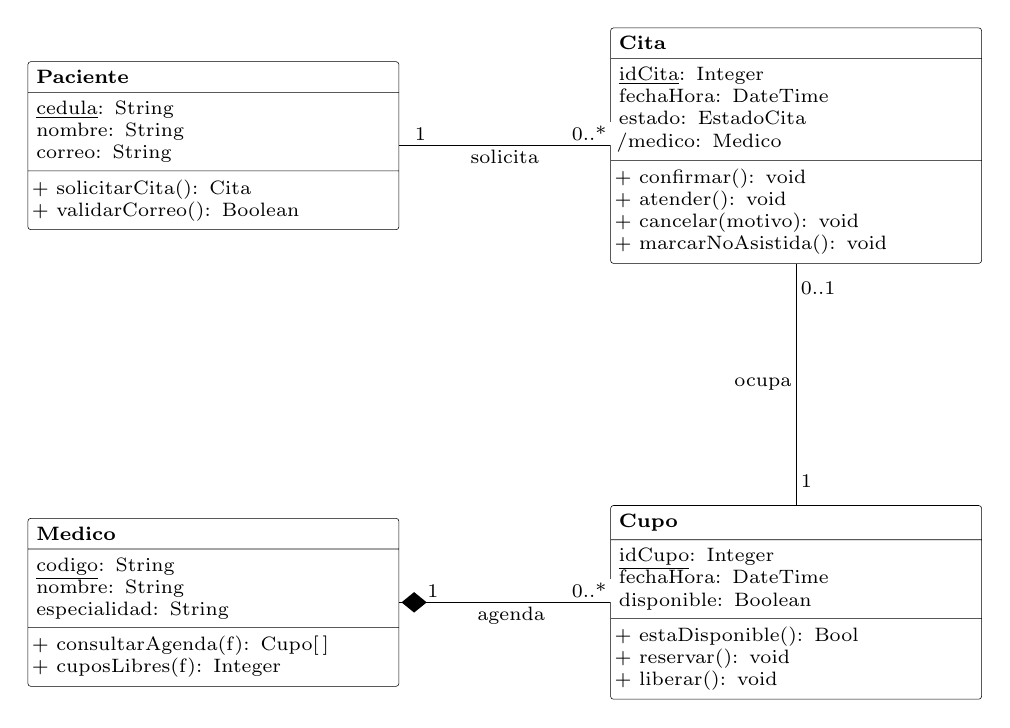
\begin{tikzpicture}

\node[clase] (paciente) at (0,0) {
  \textbf{Paciente}
  \nodepart{two}
  \underline{cedula}: String\\
  nombre: String\\
  correo: String
  \nodepart{three}
  + solicitarCita(): Cita\\
  + validarCorreo(): Boolean
};

\node[clase] (cita) at (7.4,0) {
  \textbf{Cita}
  \nodepart{two}
  \underline{idCita}: Integer\\
  fechaHora: DateTime\\
  estado: EstadoCita\\
  /medico: Medico
  \nodepart{three}
  + confirmar(): void\\
  + atender(): void\\
  + cancelar(motivo): void\\
  + marcarNoAsistida(): void
};

\node[clase] (cupo) at (7.4,-5.8) {
  \textbf{Cupo}
  \nodepart{two}
  \underline{idCupo}: Integer\\
  fechaHora: DateTime\\
  disponible: Boolean
  \nodepart{three}
  + estaDisponible(): Bool\\
  + reservar(): void\\
  + liberar(): void
};

\node[clase] (medico) at (0,-5.8) {
  \textbf{Medico}
  \nodepart{two}
  \underline{codigo}: String\\
  nombre: String\\
  especialidad: String
  \nodepart{three}
  + consultarAgenda(f): Cupo[\,]\\
  + cuposLibres(f): Integer
};

\draw[thin] (paciente.east) -- node[etiq,above,pos=0.10]{1}
                               node[etiq,above,pos=0.90]{0..*}
                               node[etiq,below,pos=0.50]{solicita} (cita.west);

\draw[thin] (cita.south) -- node[etiq,right,pos=0.10]{0..1}
                            node[etiq,right,pos=0.90]{1}
                            node[etiq,left,pos=0.50]{ocupa} (cupo.north);

\draw[thin] (medico.east) -- node[etiq,above,pos=0.16]{1}
                             node[etiq,above,pos=0.90]{0..*}
                             node[etiq,below,pos=0.53]{agenda} (cupo.west);
\fill ($(medico.east)+(0.03,0)$) -- ++(0.16,0.13) -- ++(0.16,-0.13)
      -- ++(-0.16,-0.13) -- cycle;
\end{tikzpicture}}
\end{center}
\end{respuesta}


\begin{tarea}{P2. Modelo funcional --- Diagrama de actividades UML \hfill (8 pts)}
Modele el proceso \textbf{``Agendar cita''} con un \textbf{diagrama de actividades UML} que incluya: nodo inicial, al menos una \textbf{decisi\'on} (\textsf{\textquestiondown cupo disponible?}), los dos caminos alternativos (\emph{confirmar} / \emph{notificar no disponibilidad}), su convergencia y el nodo final. Use carriles de responsabilidad si distingue actores.
\end{tarea}

\begin{respuesta}{Respuesta P2}
Se emplean dos carriles de responsabilidad, \emph{Paciente} y \emph{Sistema}. La decisi\'on
\textsf{\textquestiondown cupo disponible?} abre los dos caminos alternativos, que convergen en un nodo
de uni\'on antes del nodo final.

\begin{center}
\setlength{\fboxsep}{8pt}\colorbox{white}{%
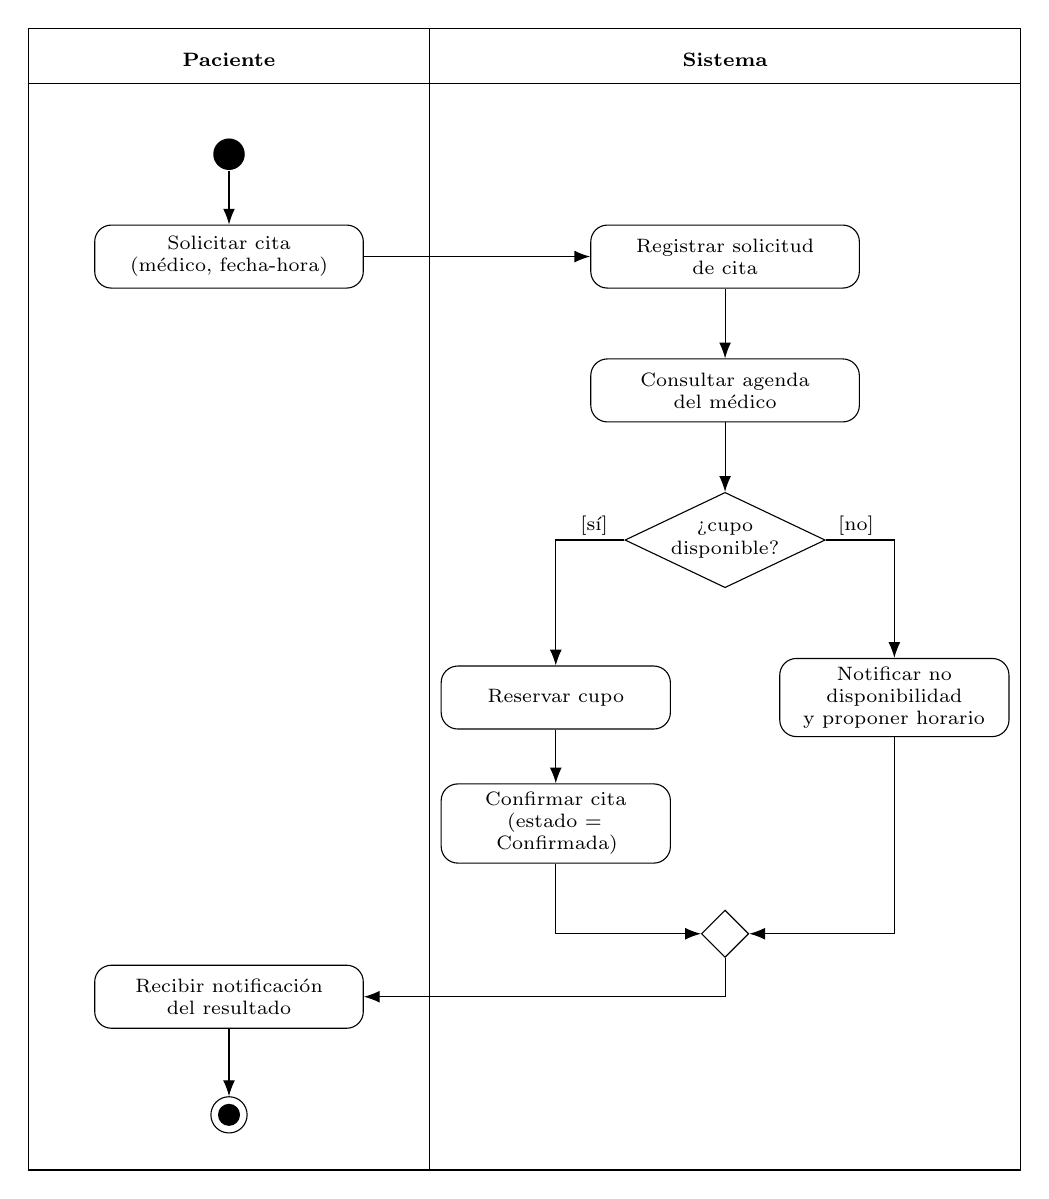
\begin{tikzpicture}
\draw[thin] (-5.4,0.9) rectangle (7.2,-13.6);
\draw[thin] (-0.3,0.9) -- (-0.3,-13.6);
\node[font=\scriptsize\bfseries] at (-2.85,0.5) {Paciente};
\node[font=\scriptsize\bfseries] at (3.45,0.5) {Sistema};
\draw[thin] (-5.4,0.2) -- (7.2,0.2);

\node[ini] (i) at (-2.85,-0.7) {};
\node[act] (solicitar) at (-2.85,-2.0) {Solicitar cita\\ (m\'edico, fecha-hora)};
\node[act] (recibir) at (-2.85,-11.4) {Recibir notificaci\'on\\ del resultado};
\node[circle,draw,minimum size=4.6mm,inner sep=0pt] (f) at (-2.85,-12.9) {};
\fill (-2.85,-12.9) circle (1.4mm);

\node[act] (registrar) at (3.45,-2.0) {Registrar solicitud\\ de cita};
\node[act] (verificar) at (3.45,-3.7) {Consultar agenda\\ del m\'edico};
\node[dec] (d) at (3.45,-5.6) {\textquestiondown cupo\\ disponible?};
\node[act,text width=2.7cm] (reservar) at (1.3,-7.6) {Reservar cupo};
\node[act,text width=2.7cm] (confirmar) at (1.3,-9.2) {Confirmar cita\\ (estado = Confirmada)};
\node[act,text width=2.7cm] (faltante) at (5.6,-7.6) {Notificar no\\ disponibilidad\\ y proponer horario};
\node[dec,aspect=1,minimum size=6mm] (m) at (3.45,-10.6) {};

\draw[flecha] (i) -- (solicitar);
\draw[flecha] (solicitar) -- (registrar);
\draw[flecha] (registrar) -- (verificar);
\draw[flecha] (verificar) -- (d);
\draw[flecha] (d.west) -| node[etiq,pos=0.22,above]{[s\'i]} (reservar);
\draw[flecha] (d.east) -| node[etiq,pos=0.22,above]{[no]} (faltante);
\draw[flecha] (reservar) -- (confirmar);
\draw[flecha] (confirmar) |- (m.west);
\draw[flecha] (faltante) |- (m.east);
\draw[flecha] (m.south) |- (recibir.east);
\draw[flecha] (recibir) -- (f);
\end{tikzpicture}}
\end{center}
\end{respuesta}


\begin{tarea}{P3. Modelo de comportamiento --- M\'aquina de estados UML \hfill (8 pts)}
Elabore la \textbf{m\'aquina de estados UML} del ciclo de vida de una \textsf{Cita} (p.\,ej. \textsf{Solicitada}, \textsf{Confirmada}, \textsf{Atendida}, \textsf{Cancelada}, \textsf{No asistida}). Etiquete cada \textbf{transici\'on} con su \textbf{evento}, incluya al menos una \textbf{condici\'on de guarda} y marque el estado final de aceptaci\'on. Se valora el uso de un superestado (statechart) para factorizar la transici\'on \emph{cancelar}.
\end{tarea}

\begin{respuesta}{Respuesta P3}
El superestado \textsf{CitaVigente} factoriza la transici\'on \textsf{cancelar}: en lugar de repetirla
en cada estado interno, se dibuja una sola vez desde el borde del superestado con la guarda
\textsf{[estado $\neq$ Atendida]}. \textsf{Atendida} es el estado final de aceptaci\'on;
\textsf{Cancelada} y \textsf{No asistida} son finales alternativos.

\begin{center}
\setlength{\fboxsep}{8pt}\colorbox{white}{%
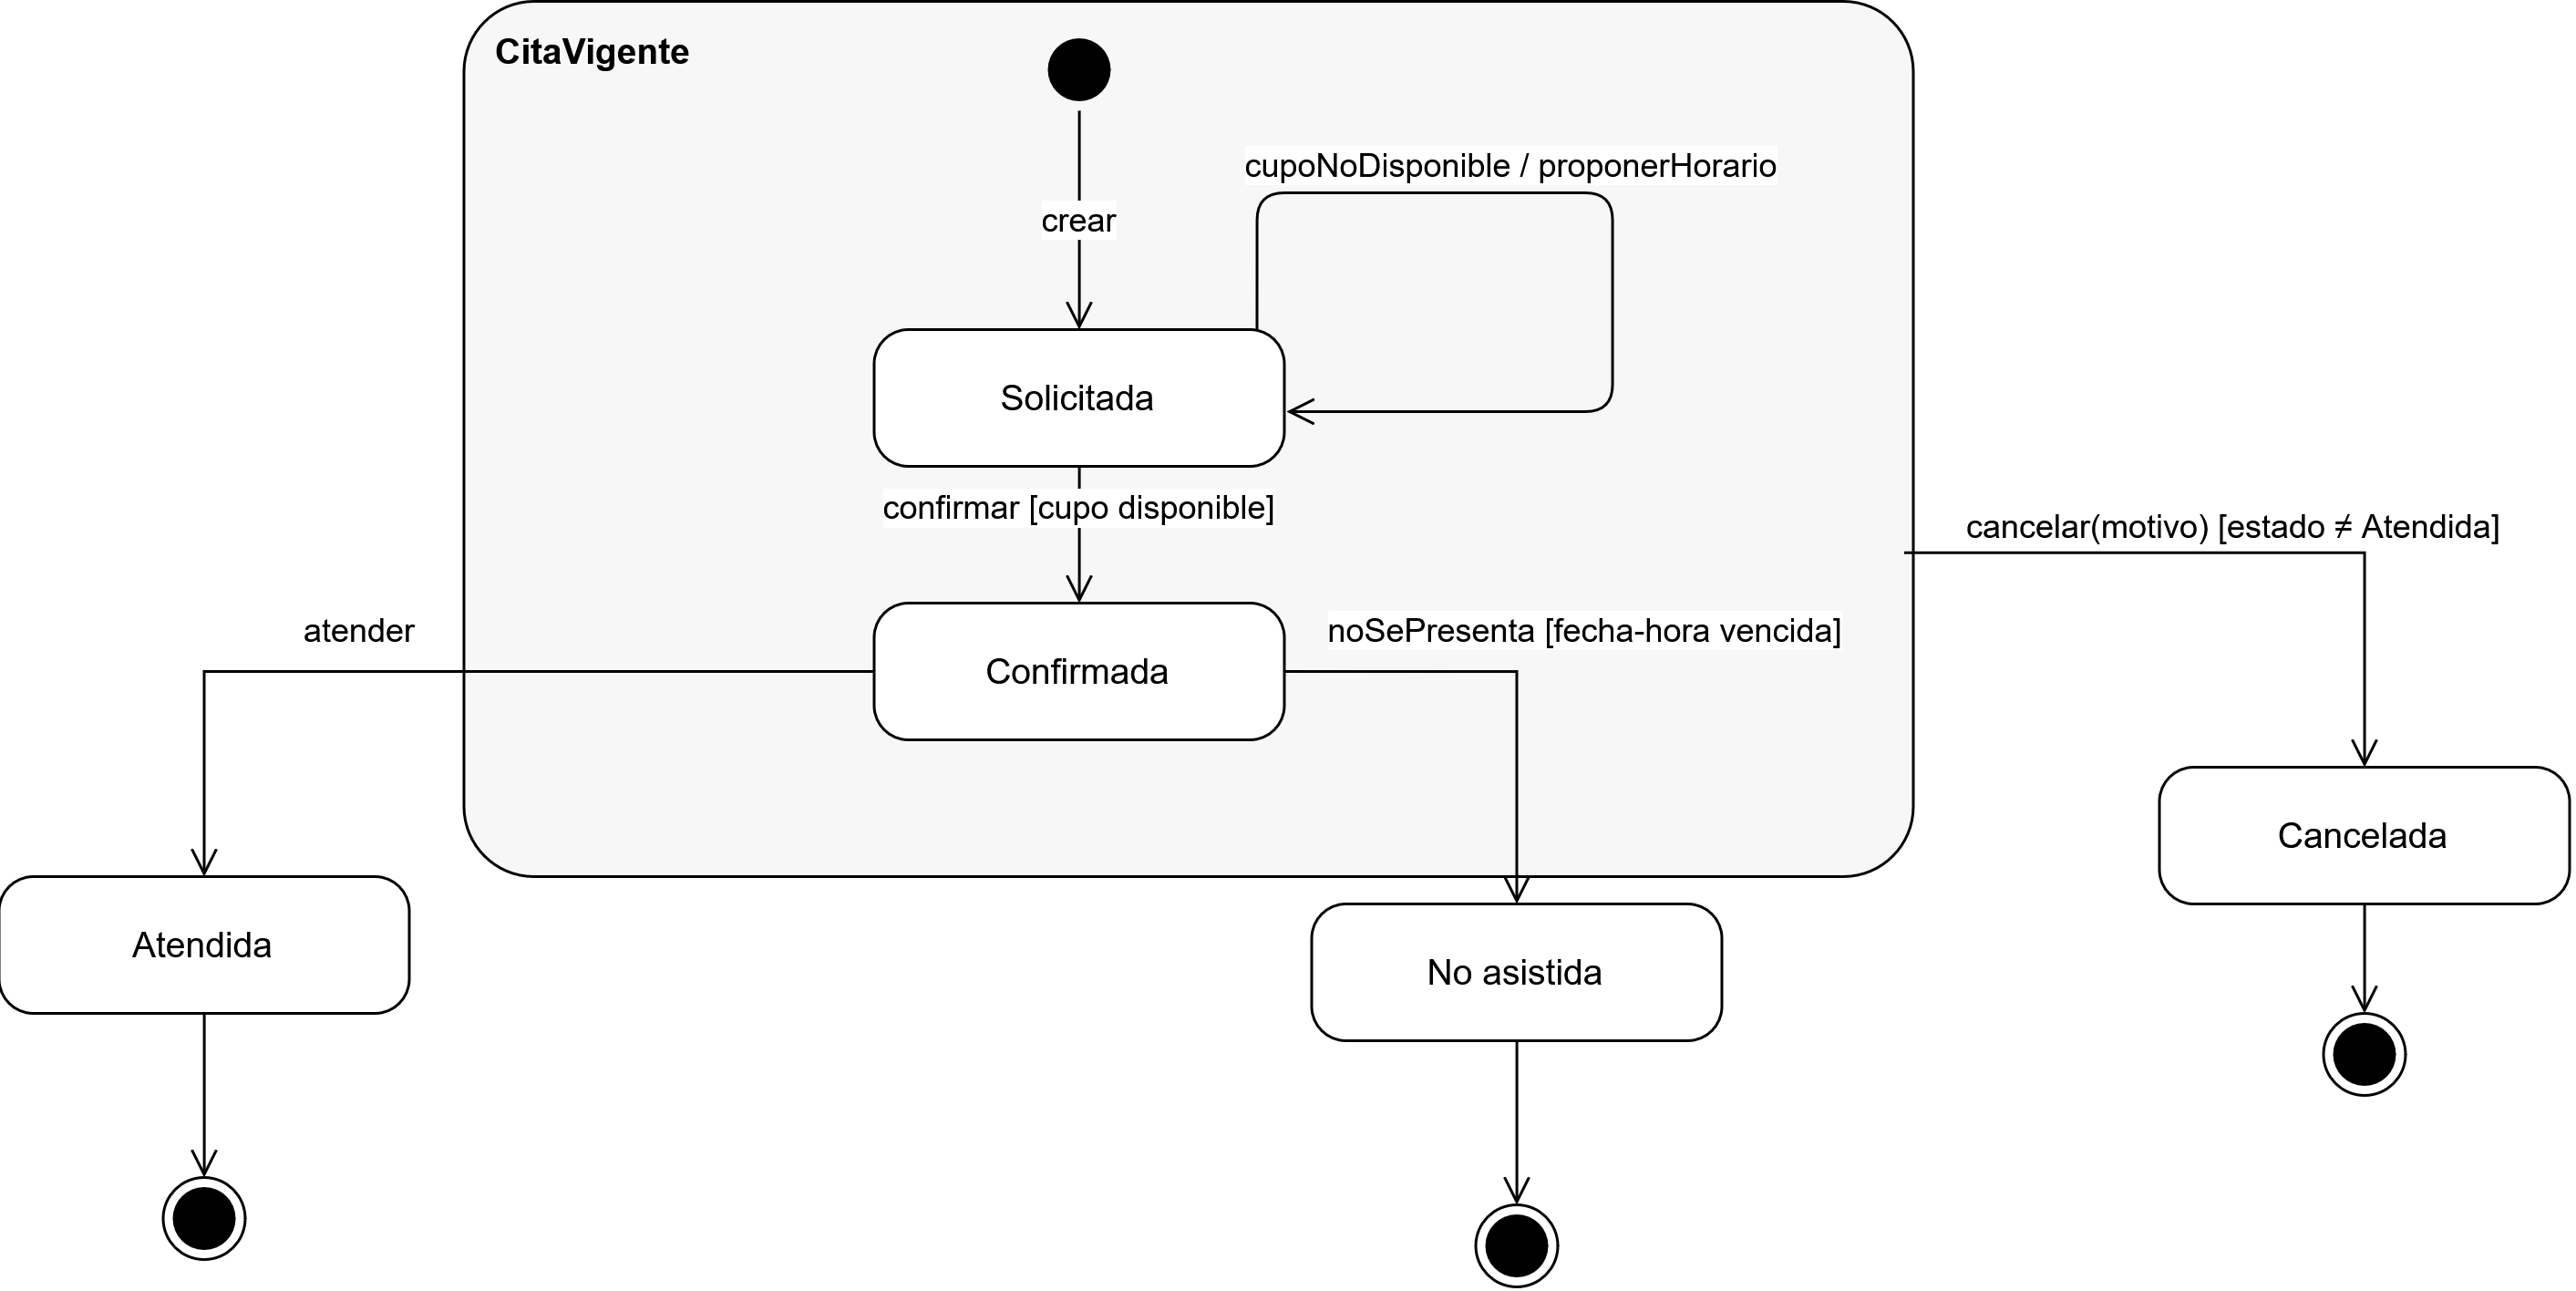
\includegraphics[width=0.92\linewidth]{figuras/P3-maquina-estados-cita_drawio.png}}
\end{center}
\end{respuesta}


\begin{tarea}{P4. Consistencia entre las tres perspectivas \hfill (7 pts)}
Elabore una \textbf{tabla de verificaci\'on cruzada} que relacione cada \textbf{evento} de P3 con la \textbf{funci\'on/acci\'on} de P2 que lo realiza y con la \textbf{entidad o atributo} de P1 que modifica. \textbf{Detecte al menos una inconsistencia} entre los modelos (evento sin funci\'on, entidad sin clase, etc.), \textbf{documente} el defecto y \textbf{corrija} el modelo afectado.
\end{tarea}

\begin{respuesta}{Respuesta P4}
\textbf{Tabla de verificaci\'on cruzada.}

\begin{center}\footnotesize
\begin{tabularx}{\linewidth}{@{}L{3.0cm} X X@{}}
\toprule
\hd{Evento (P3)} & \hd{Funci\'on/acci\'on que lo realiza (P2)} & \hd{Entidad/atributo que modifica (P1)}\\
\midrule
\textsf{crear} & Registrar solicitud de cita & \textsf{Cita.idCita}, \textsf{Cita.fechaHora},
\textsf{Cita.estado} $\leftarrow$ Solicitada\\
\rowcolor{rowgray}
\textsf{cupoNoDisponible} & Notificar no disponibilidad y proponer otro horario & Ninguno (solo
notificaci\'on); consulta \textsf{Cupo.disponible}\\
\textsf{confirmar} [cupo disponible] & Consultar agenda $\rightarrow$ Reservar cupo $\rightarrow$
Confirmar cita & \textsf{Cupo.disponible} $\leftarrow$ falso; \textsf{Cita.estado} $\leftarrow$
Confirmada\\
\rowcolor{rowgray}
\textsf{atender} & \textbf{Sin funci\'on asociada en P2} & \textsf{Cita.estado} $\leftarrow$ Atendida\\
\textsf{noSePresenta} & \textbf{Sin funci\'on asociada en P2} & \textsf{Cita.estado} $\leftarrow$
No asistida\\
\rowcolor{rowgray}
\textsf{cancelar(motivo)} & \textbf{Sin funci\'on asociada en P2} & \textsf{Cita.estado} $\leftarrow$
Cancelada; \textsf{Cupo.disponible} $\leftarrow$ verdadero\\
\bottomrule
\end{tabularx}
\end{center}

\textbf{Correcci\'on aplicada.} Se corrigen dos modelos de forma coordinada: en \textbf{P1} se
a\~naden las operaciones \textsf{Cita.cancelar(motivo)} y \textsf{Cupo.liberar()} (ya incorporadas en
la figura de P1); en \textbf{P2} se agrega el fragmento de actividad ``Cancelar cita'' que cierra la
traza evento $\rightarrow$ funci\'on $\rightarrow$ entidad.

\begin{center}
\setlength{\fboxsep}{8pt}\colorbox{white}{%
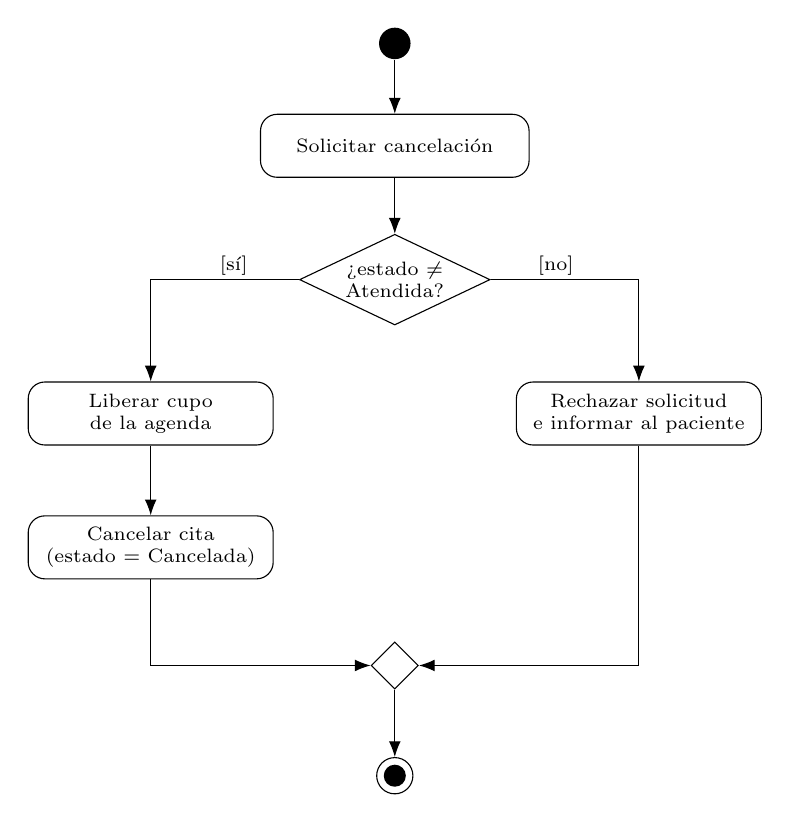
\begin{tikzpicture}
\node[ini] (i) at (0,0) {};
\node[act] (sol) at (0,-1.3) {Solicitar cancelaci\'on};
\node[dec] (d) at (0,-3.0) {\textquestiondown estado $\neq$\\ Atendida?};
\node[act,text width=2.9cm] (lib) at (-3.1,-4.7) {Liberar cupo\\ de la agenda};
\node[act,text width=2.9cm] (canc) at (-3.1,-6.4) {Cancelar cita\\ (estado = Cancelada)};
\node[act,text width=2.9cm] (rech) at (3.1,-4.7) {Rechazar solicitud\\ e informar al paciente};
\node[dec,aspect=1,minimum size=6mm] (m) at (0,-7.9) {};
\node[circle,draw,minimum size=4.6mm,inner sep=0pt] (f) at (0,-9.3) {};
\fill (0,-9.3) circle (1.4mm);

\draw[flecha] (i) -- (sol);
\draw[flecha] (sol) -- (d);
\draw[flecha] (d.west) -| node[etiq,pos=0.22,above]{[s\'i]} (lib);
\draw[flecha] (d.east) -| node[etiq,pos=0.22,above]{[no]} (rech);
\draw[flecha] (lib) -- (canc);
\draw[flecha] (canc) |- (m.west);
\draw[flecha] (rech) |- (m.east);
\draw[flecha] (m) -- (f);
\end{tikzpicture}}
\end{center}
\end{respuesta}


\begin{tarea}{P5. Especificaci\'on de requisitos con esquema de atributos \hfill (10 pts)}
Redacte \textbf{4 requisitos}: \textbf{2 funcionales} y \textbf{2 no funcionales}. Cada requisito no funcional debe \textbf{nombrar una caracter\'istica de \textit{ISO/IEC} 25010:2023} (p.\,ej. Eficiencia de desempe\~no, Seguridad), fijar una \textbf{m\'etrica} y un \textbf{umbral} (p.\,ej. ``agendar la cita en $<$ 3 s''). Para cada requisito complete un \textbf{esquema de atributos}: identificador, prioridad, estado, fuente, estabilidad, versi\'on y m\'etodo de verificaci\'on.
\end{tarea}

\begin{respuesta}{Respuesta P5}
Cuatro requisitos en versi\'on 1.0: dos funcionales y dos no funcionales, cada uno de estos \'ultimos
con su caracter\'istica de \textit{ISO/IEC} 25010:2023, su m\'etrica y su umbral.

\begin{center}\footnotesize
\begin{tabularx}{\linewidth}{@{}L{3.1cm} X@{}}
\toprule
\multicolumn{2}{@{}l}{\hm{RF-01 --- Agendamiento de cita con verificaci\'on de cupo}}\\
\midrule
Enunciado & El sistema debe registrar la solicitud de cita de un paciente para un m\'edico y una
fecha-hora determinados, y verificar la disponibilidad del cupo correspondiente en la agenda de ese
m\'edico. Si el cupo est\'a disponible, debe reservarlo y dejar la cita en estado
\textsf{Confirmada}; en caso contrario, debe notificar la no disponibilidad y proponer los tres cupos
libres m\'as pr\'oximos del mismo m\'edico.\\
\rowcolor{rowgray}
Identificador & RF-01\\
Prioridad & Alta\\
\rowcolor{rowgray}
Estado & Aprobado\\
Fuente & Caso de negocio, p\'arrafo 2\\
\rowcolor{rowgray}
Estabilidad & Alta\\
Versi\'on & 1.0\\
\rowcolor{rowgray}
M\'etodo de verificaci\'on & Prueba funcional sobre cupo disponible y cupo ocupado\\
\bottomrule
\end{tabularx}
\end{center}

\begin{center}\footnotesize
\begin{tabularx}{\linewidth}{@{}L{3.1cm} X@{}}
\toprule
\multicolumn{2}{@{}l}{\hm{RF-02 --- Cancelaci\'on de cita no atendida}}\\
\midrule
Enunciado & El paciente titular de la cita, o un recepcionista autorizado, debe poder cancelarla
mientras su estado sea distinto de \textsf{Atendida}. Al hacerlo, el sistema debe liberar el cupo
reservado y registrar el motivo de la cancelaci\'on.\\
\rowcolor{rowgray}
Identificador & RF-02\\
Prioridad & Media\\
\rowcolor{rowgray}
Estado & Propuesto\\
Fuente & Caso de negocio, p\'arrafo 2\\
\rowcolor{rowgray}
Estabilidad & Media\\
Versi\'on & 1.0\\
\rowcolor{rowgray}
M\'etodo de verificaci\'on & Prueba funcional sobre cita confirmada y sobre cita atendida\\
\bottomrule
\end{tabularx}
\end{center}

\begin{center}\footnotesize
\begin{tabularx}{\linewidth}{@{}L{3.1cm} X@{}}
\toprule
\multicolumn{2}{@{}l}{\hm{RNF-01 --- Tiempo de agendamiento de la cita}}\\
\midrule
Enunciado & El sistema debe completar la transacci\'on ``agendar cita'' en menos de 3 s en el
percentil 95, medido en el servidor de aplicaci\'on, con 200 usuarios concurrentes y una agenda de 500
m\'edicos.\\
\rowcolor{rowgray}
Caracter\'istica 25010:2023 & Eficiencia de desempe\~no\\
M\'etrica & Tiempo de respuesta de la transacci\'on\\
\rowcolor{rowgray}
Umbral & $<$ 3 seg\\
Identificador & RNF-01\\
\rowcolor{rowgray}
Prioridad & Alta\\
Estado & Propuesto\\
\rowcolor{rowgray}
Fuente & Caso de negocio\\
Estabilidad & Media\\
\rowcolor{rowgray}
Versi\'on & 1.0\\
M\'etodo de verificaci\'on & Prueba de carga con 200 usuarios concurrentes durante 10 minutos\\
\bottomrule
\end{tabularx}
\end{center}

\begin{center}\footnotesize
\begin{tabularx}{\linewidth}{@{}L{3.1cm} X@{}}
\toprule
\multicolumn{2}{@{}l}{\hm{RNF-02 --- Protecci\'on de los datos personales del paciente}}\\
\midrule
Enunciado & El sistema debe almacenar cifrados con AES-256 el 100\,\% de los campos personales del
paciente (c\'edula, nombre y correo) y transmitirlos \'unicamente sobre TLS 1.3.\\
\rowcolor{rowgray}
Caracter\'istica 25010:2023 & Seguridad\\
M\'etrica & Porcentaje de campos personales\\
\rowcolor{rowgray}
Umbral & 100\,\%\\
Identificador & RNF-02\\
\rowcolor{rowgray}
Prioridad & Alta\\
Estado & Propuesto\\
\rowcolor{rowgray}
Fuente & Caso de negocio\\
Estabilidad & Alta\\
\rowcolor{rowgray}
Versi\'on & 1.0\\
M\'etodo de verificaci\'on & Inspecci\'on de la configuraci\'on de cifrado y captura de tr\'afico\\
\bottomrule
\end{tabularx}
\end{center}

\end{respuesta}


\begin{tarea}{P6. Priorizaci\'on MoSCoW \hfill (5 pts)}
Clasifique los 4 requisitos de P5 en las categor\'ias \textbf{MoSCoW} (\textit{Must / Should / Could / Won't have this time}) y \textbf{justifique} brevemente cada asignaci\'on en funci\'on del valor y la viabilidad. Al menos un requisito debe ser \textit{Must have}.
\end{tarea}

\begin{tarea}{P7. Validaci\'on por inspecci\'on (lista de comprobaci\'on 29148) \hfill (8 pts)}
Aplique a los requisitos de P5 una \textbf{lista de comprobaci\'on} derivada de las propiedades de \textit{ISO/IEC/IEEE} 29148 (no ambiguo, completo, singular, verificable, factible). \textbf{Registre los defectos detectados sin corregirlos en el momento} (separar identificaci\'on de correcci\'on) y, en un segundo paso, presente el \textbf{retrabajo} con los requisitos corregidos.
\end{tarea}

\begin{tarea}{P8. Pruebas de aceptaci\'on trazadas \hfill (6 pts)}
Defina \textbf{una prueba de aceptaci\'on por requisito} (4 en total), indicando su \textbf{tipo} (funcional, no funcional o regresi\'on), sus \textbf{entradas}, el \textbf{criterio de \'exito} y el \textbf{requisito al que traza}. Cada prueba debe enlazar expl\'icitamente con al menos un requisito de P5.
\end{tarea}

\begin{tarea}{P9. Matriz de trazabilidad \hfill (6 pts)}
Construya la \textbf{matriz de trazabilidad} que cruce los requisitos con: su \textbf{fuente} (traza hacia atr\'as) y sus \textbf{modelos y pruebas de aceptaci\'on} (traza hacia adelante). Marque tambi\'en al menos una dependencia \textbf{horizontal} entre requisitos e \textbf{identifique} cualquier requisito hu\'erfano (sin prueba o sin modelo asociado).
\end{tarea}

\begin{tarea}{P10. Gesti\'on del cambio y l\'inea base \hfill (4 pts)}
Simule \textbf{una solicitud de cambio} sobre un requisito: reg\'istrela, \textbf{analice su impacto} usando la matriz de P9, indique la \textbf{decisi\'on del CCB} (aprobada/rechazada/diferida) y \textbf{actualice la versi\'on} del requisito. Finalmente, declare una \textbf{l\'inea base}: liste la \textbf{configuraci\'on} (versiones coherentes de ERS, modelos, matriz y pruebas) que se congela.
\end{tarea}

% #####################################################################
\section{Rúbrica de evaluaci\'on}

La calificaci\'on total es de \textbf{100 puntos}, distribuidos en \textbf{30\%} para el cuestionario rendido en el LMS (SGA) y \textbf{70\%} para el desarrollo de la prueba pr\'actica. Los \textbf{criterios de piso} de la Secci\'on~1 se aplican \emph{antes} de sumar puntos: si alguno se incumple, la calificaci\'on final es \textbf{CERO}, con independencia de los puntos logrados en cada criterio.

\begin{concepto}{Escala de niveles de logro (se aplica a cada criterio de la prueba pr\'actica)}
\textbf{Logrado (100\% del peso):} el producto cumple \'integramente lo solicitado, es correcto y consistente. \quad \textbf{Parcial (60\%):} cumple lo esencial pero con omisiones o errores menores. \quad \textbf{Insuficiente (30\%):} entrega incompleta o con errores conceptuales relevantes. \quad \textbf{No entregado (0\%):} ausente o no evaluable.
\end{concepto}

% ── Componente SGA 30% ──
\begin{table}[htbp]
	\centering
	\caption{Componente 1 --- Cuestionario en el LMS (SGA). Peso: 30 puntos.}
	\small
	\begin{tabularx}{\linewidth}{@{}L{4.6cm} C{1.6cm} X@{}}
		\toprule
		\hd{Criterio} & \hd{Peso} & \hd{Evidencia requerida}\\
		\midrule
		Nota obtenida en el cuestionario del SGA & 20 pts & Puntaje autocalificado por el LMS, proporcional al porcentaje de aciertos.\\
		\rowcolor{rowgray}
		Captura del \emph{resumen} del cuestionario en la car\'atula & 5 pts & Imagen legible del resumen de resultados incrustada en la portada del PDF.\\
		Captura de la \emph{evaluaci\'on} (intento) en la car\'atula & 5 pts & Imagen legible del intento/evaluaci\'on incrustada en la portada del PDF.\\
		\bottomrule
	\end{tabularx}
\end{table}

% ── Componente practica 70% (landscape) ──
\begin{landscape}
\begin{table}[htbp]
	\centering
	\caption{Componente 2 --- Desarrollo de la prueba pr\'actica. Peso: 70 puntos. (Logrado 100\% / Parcial 60\% / Insuficiente 30\% / No entregado 0\% del peso indicado.)}
	\scriptsize
	\renewcommand{\arraystretch}{1.2}
	\begin{tabularx}{\linewidth}{@{}L{3.0cm} C{0.9cm} X X X@{}}
		\toprule
		\hd{Criterio (tarea)} & \hd{Peso} & \hd{Logrado (100\%)} & \hd{Parcial (60\%)} & \hd{Insuficiente (30\%)}\\
		\midrule
		P1. Diagrama de clases UML & 8 & Clases, atributos tipados, operaciones y multiplicidades correctas y coherentes con el caso. & Faltan operaciones o alguna multiplicidad; estructura b\'asica correcta. & Clases incompletas o sin multiplicidades; errores de modelado.\\
		\rowcolor{rowgray}
		P2. Diagrama de actividades UML & 8 & Decisi\'on de \textit{cupo}, ambos caminos, convergencia y nodo final bien modelados. & Flujo correcto pero sin decisi\'on o sin convergencia expl\'icita. & Secuencia lineal sin l\'ogica de control del caso.\\
		P3. M\'aquina de estados UML & 8 & Estados, eventos, guarda y estado final; superestado bien usado. & Estados y eventos correctos, sin guarda o sin estado final. & Estados incompletos o transiciones sin evento.\\
		\rowcolor{rowgray}
		P4. Consistencia entre perspectivas & 7 & Tabla cruzada completa; inconsistencia detectada, documentada y corregida. & Tabla parcial o inconsistencia detectada pero no corregida. & Tabla ausente o sin an\'alisis de correspondencia.\\
		P5. Requisitos con esquema de atributos & 10 & 4 requisitos (2 F, 2 NF) con caracter\'istica 25010, m\'etrica, umbral y atributos completos. & Requisitos correctos con atributos incompletos o sin umbral. & Requisitos ambiguos o sin esquema de atributos.\\
		\rowcolor{rowgray}
		P6. Priorizaci\'on MoSCoW & 5 & Cuatro requisitos clasificados y justificados; al menos un \textit{Must}. & Clasificaci\'on correcta con justificaci\'on d\'ebil. & Clasificaci\'on sin justificar o mal aplicada.\\
		P7. Inspecci\'on 29148 (defectos + retrabajo) & 8 & Checklist aplicada; defectos registrados sin corregir y retrabajo presentado. & Defectos detectados sin retrabajo, o correcci\'on mezclada con detecci\'on. & Sin checklist o sin evidencia de defectos.\\
		\rowcolor{rowgray}
		P8. Pruebas de aceptaci\'on trazadas & 6 & 4 pruebas con tipo, entradas, criterio de \'exito y traza al requisito. & Pruebas sin tipo o sin criterio de \'exito claro. & Pruebas sin traza a requisitos.\\
		P9. Matriz de trazabilidad & 6 & Trazas hacia atr\'as, adelante y horizontal; hu\'erfanos identificados. & Matriz parcial (solo un sentido de traza). & Matriz ausente o sin correspondencias reales.\\
		\rowcolor{rowgray}
		P10. Gesti\'on del cambio y l\'inea base & 4 & Solicitud, impacto, decisi\'on CCB, versi\'on y configuraci\'on/baseline declarada. & Cambio registrado sin impacto o sin baseline. & Sin proceso de cambio ni l\'inea base.\\
		\midrule
		\hg{Total del componente pr\'actico} & \hg{70} & \multicolumn{3}{c}{\cellcolor{lightgray}\small\color{darkblue} Suma de puntos logrados por nivel en cada criterio.}\\
		\bottomrule
	\end{tabularx}
\end{table}
\end{landscape}

\begin{table}[htbp]
	\centering
	\caption{Resumen de ponderaci\'on final.}
	\small
	\begin{tabularx}{\linewidth}{@{}X C{2.4cm} C{3.0cm}@{}}
		\toprule
		\hd{Componente} & \hd{Peso} & \hd{Condici\'on}\\
		\midrule
		Cuestionario en el LMS (SGA) + capturas en car\'atula & 30 pts & Sujeto a criterios de piso\\
		\rowcolor{rowgray}
		Desarrollo de la prueba pr\'actica (P1--P10) & 70 pts & Sujeto a criterios de piso\\
		\midrule
		\hg{Total} & \hg{100 pts} & \hg{CERO si se incumple un criterio de piso}\\
		\bottomrule
	\end{tabularx}
\end{table}

% #####################################################################
\section{Marco normativo de referencia}

Esta prueba operacionaliza las propiedades de calidad de la norma \textit{ISO/IEC/IEEE} 29148:2018 \citep{iso29148_2018} y el modelo de calidad de producto \textit{ISO/IEC} 25010:2023 \citep{iso25010_2023}, junto con las t\'ecnicas de validaci\'on y gesti\'on descritas por Pohl \citep{pohl_2010}, la inspecci\'on formal de Fagan \citep{fagan_1976} y las buenas pr\'acticas recogidas en la gu\'ia SWEBOK v4 \citep{swebok_v4_2024}. Las notaciones de modelado siguen la especificaci\'on \textit{OMG UML} 2.5.1 \citep{omg_uml_2017}.

\vspace{4pt}
\renewcommand{\refname}{Referencias}
\bibliographystyle{plainnat}
\bibliography{referencias}

\end{document}
